\documentclass{article} 
\usepackage{tikz}
\begin{document} 
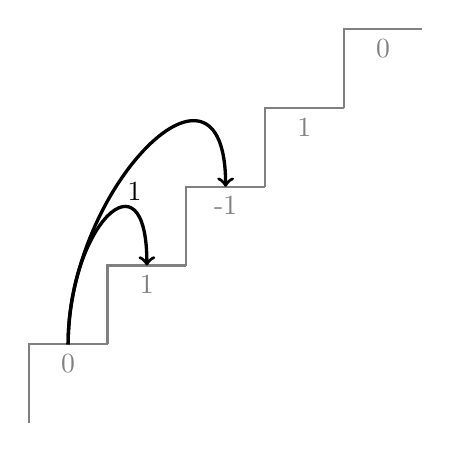
\begin{tikzpicture}[node distance={10mm}, very thick, main/.style = {thick,shorten <=1mm,dash pattern=on 8mm off 2mm}] 
\draw[gray, thick] (-3,-3) |- (-2,-2) node [pos=.75, below] (1) {0};
\draw[gray, thick] (-2,-2) |- (-1,-1) node [pos=.75, below] (2) {1};
\draw[gray, thick] (-1,-1) |- (0,0) node [pos=.75, below] (3) {-1};
\draw[gray, thick] (0,0) |- (1,1) node [pos=.75, below] (4) {1};
\draw[gray, thick] (1,1) |- (2,2) node [pos=.75, below] (5) {0};
\draw[->] (1.north) .. controls +(up:15mm) and +(up:15mm) .. (2.north) node [pos=.75, above] {1};
\draw[->] (1.north) .. controls +(up:20mm) and +(up:20mm) .. (3.north);
\end{tikzpicture} 
\end{document}